\documentclass{beamer}
\usepackage{hyperref}
\usepackage[T1]{fontenc}
\UseRawInputEncoding
\usepackage[utf8]{inputenc}
\usepackage[T1]{fontenc}
\usepackage[francais]{babel}
\usepackage{graphicx} 
\usepackage{hyperref}
\usepackage{xcolor}
\usepackage{array,multirow,makecell}
\usepackage{eso-pic}
% Cannot enable in Xelatex
\usepackage{pgfpages}
% \setbeameroption{hide notes} % Only slides
% \setbeameroption{show only notes} % Only notes
% \setbeameroption{show notes on second screen}

% other packages
\usepackage{latexsym,amsmath,xcolor,multicol,booktabs,calligra}
\usepackage{graphicx,listings,stackengine}

%% Enable only in Xelatex
% \usepackage{pstricks}

\author{EL MEHDI EL AINE}
\title{Présentation du PFE}
\subtitle{EasyGio}
\institute [École supérieure de technologie Safi, GI] {École supérieure de technologie Safi\\Université Cadi Ayyad}
\date{21 juin 2021}
\usepackage{QUT}

% defs
\def\cmd#1{\texttt{\color{red}\footnotesize $\backslash$#1}}
\def\env#1{\texttt{\color{blue}\footnotesize #1}}
\definecolor{deepblue}{rgb}{0,0,0.5}
\definecolor{deepred}{rgb}{0.6,0,0}
\definecolor{deepgreen}{rgb}{0,0.5,0}
\definecolor{halfgray}{gray}{0.55}

\lstset{
    basicstyle=\ttfamily\small,
    keywordstyle=\bfseries\color{deepblue},
    emphstyle=\ttfamily\color{deepred},    % Custom highlighting style
    stringstyle=\color{deepgreen},
    numbers=left,
    numberstyle=\small\color{halfgray},
    rulesepcolor=\color{red!20!green!20!blue!20},
    frame=shadowbox,
}


\begin{document}

\begin{frame}
    \titlepage
    \centering
    
\includegraphics[width=0.2\textwidth]{pic/logox2.png}
\end{frame}
\begin{frame}
    \tableofcontents[sectionstyle=show,subsectionstyle=show/shaded/hide,subsubsectionstyle=show/shaded/hide]
\end{frame}
\section{Introduction}
\begin{frame}{Problématique}
La géométrie a de tout temps, souffert d'une réputation de matière difficile! Des droits parallèles que l'on n'arrive pas à tracer, en passant par une intersection difficile à déterminer, ou des cercles peu assurés, la géométrie est parfois repoussée par les élèves.
\begin{center}
    
\includegraphics[width=5cm]{pic/prob.jpg}
\end{center}
\end{frame}
\begin{frame}{Solution}
Afin d'y remédier à tous ses problèmes, nous avons assigné à notre étude la solution qui consiste à développer une application bureau EasyGio pour aider les élèves du lycée et leurs enseignants à illustrer les notions de géométrie surtout dans l’espace au niveau du lycée.
\begin{center}
    
\includegraphics[width=5cm]{pic/solu.jpg}
\end{center}
\end{frame}
\section{Description du projet}
\begin{frame}{Description générale du projet}
EasyGio est une application bureau développer avec Asymptote et Python,une application rapide, simple et rapidement accessible.
\begin{center}
    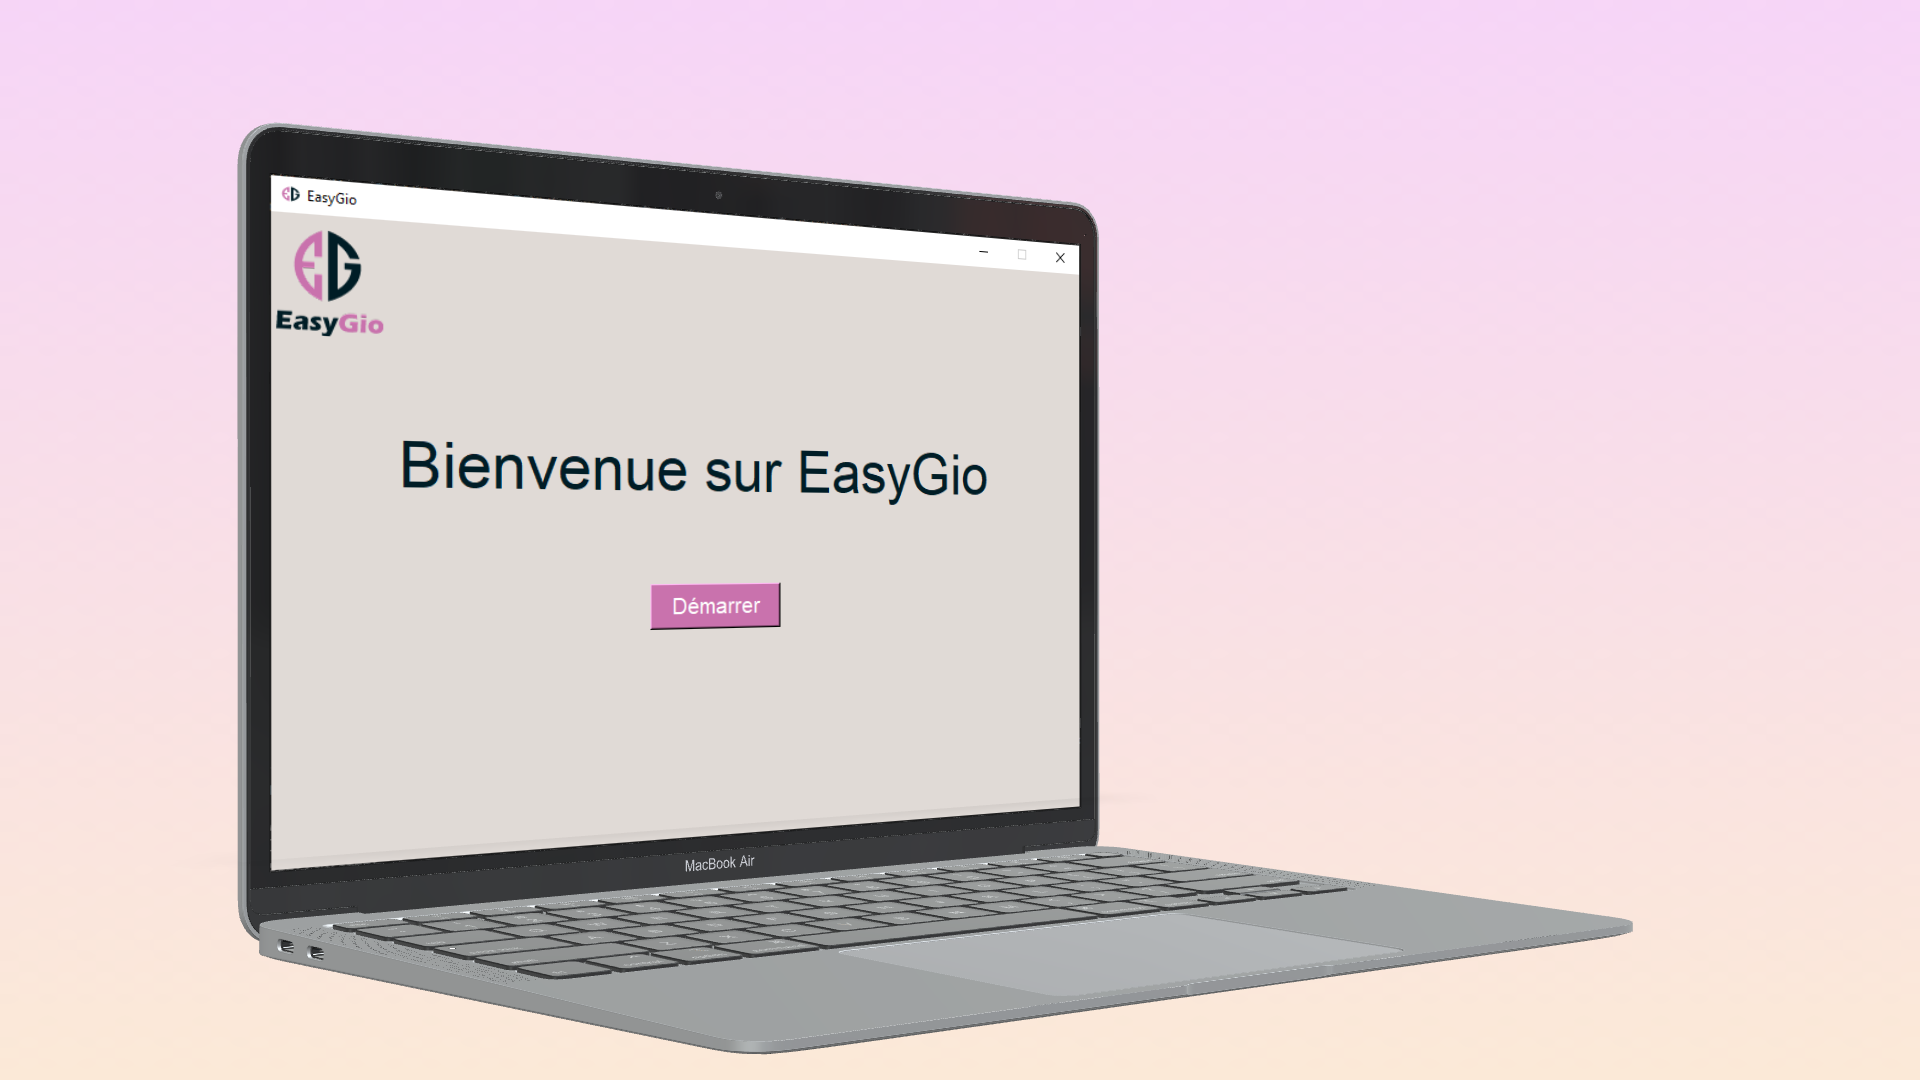
\includegraphics[width=9cm]{pic/previewed.png}
\end{center}
\end{frame}
\begin{frame}{Les services d'EasyGio}
EasyGio permet à l'utilisateur d'obtenir:
\begin{itemize}[<+-| alert@+>]
    \item Les courbes des fonctions.
    \item Des multiples graphes géométriques 2D.
    \item Des différents figures en 3D.
\end{itemize}
    \centering
    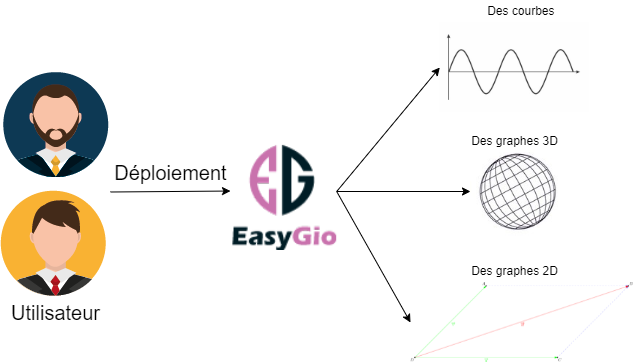
\includegraphics[width=9cm]{pic/EasyGioServices.png}
\end{frame}
\section{Analyse et conception }
\subsection{Analyse des besoins}
\begin{frame}{Diagramme d'Ishikawa}
\begin{center}
    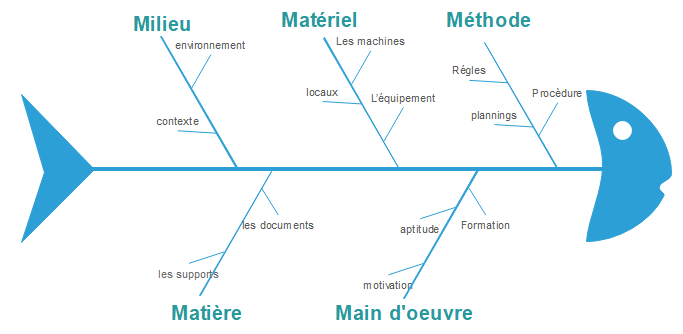
\includegraphics[width=11cm]{pic/Ishikawa.PNG}
\end{center}
\end{frame}
\begin{frame}{Diagramme de Gantt}
\begin{center}
     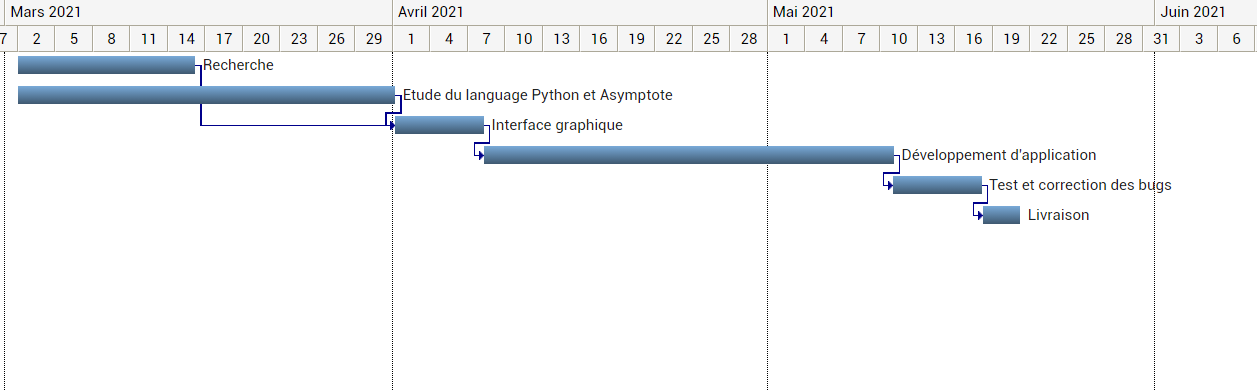
\includegraphics[width=10cm]{pic/Gantt.PNG}   
\end{center}
\end{frame}
\begin{frame}{Diagramme de cas d'utilisation}
\begin{center}
    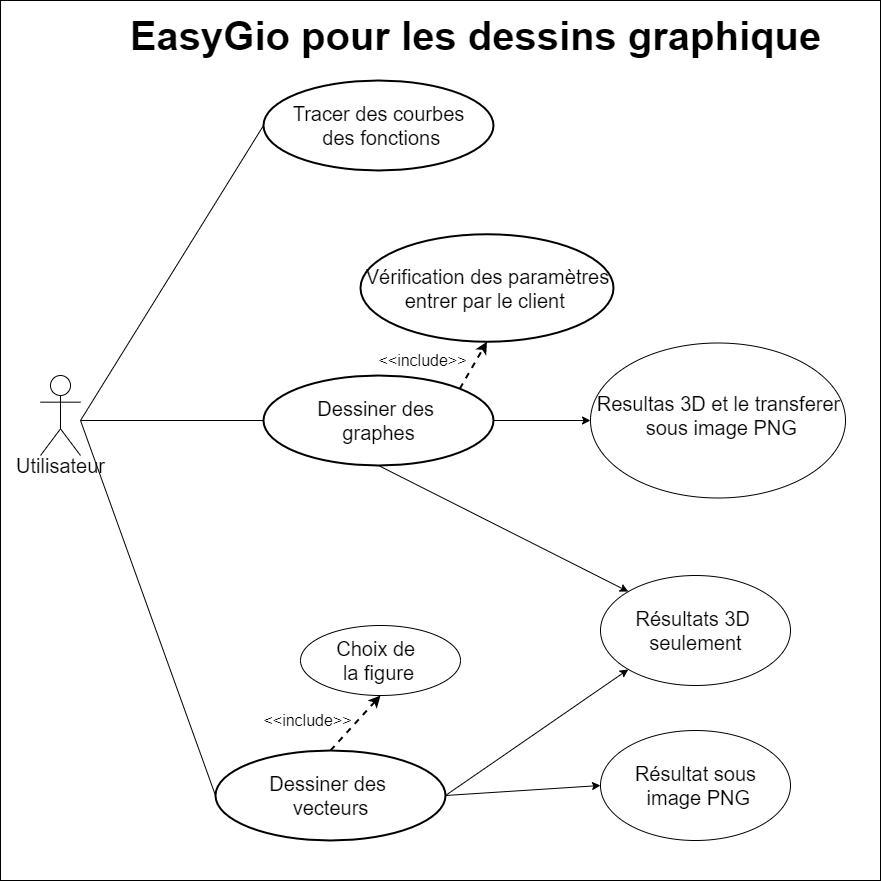
\includegraphics[width=6.6cm]{pic/MY UML.png}
\end{center}
\end{frame}
\subsection{Conception}
\begin{frame}{Description textuelle détaillé de cas d'utilisation}
 \begin{center}
     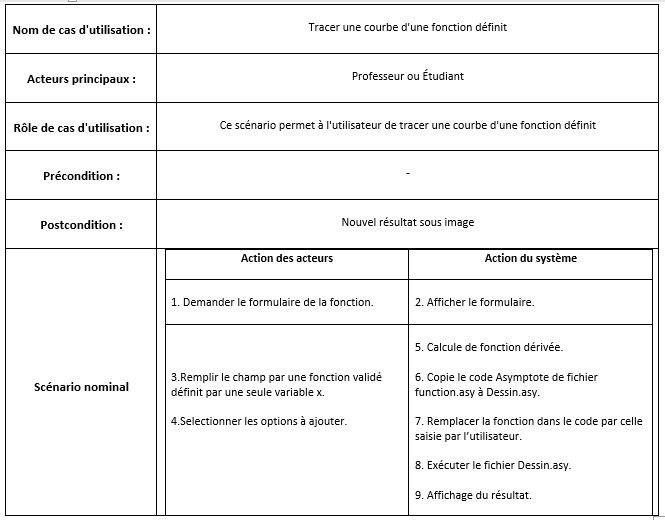
\includegraphics[width=9cm]{pic/TableDescActi.PNG} 
 \end{center}  
\end{frame}
\begin{frame}{Diagramme de séquence}
\begin{center}
    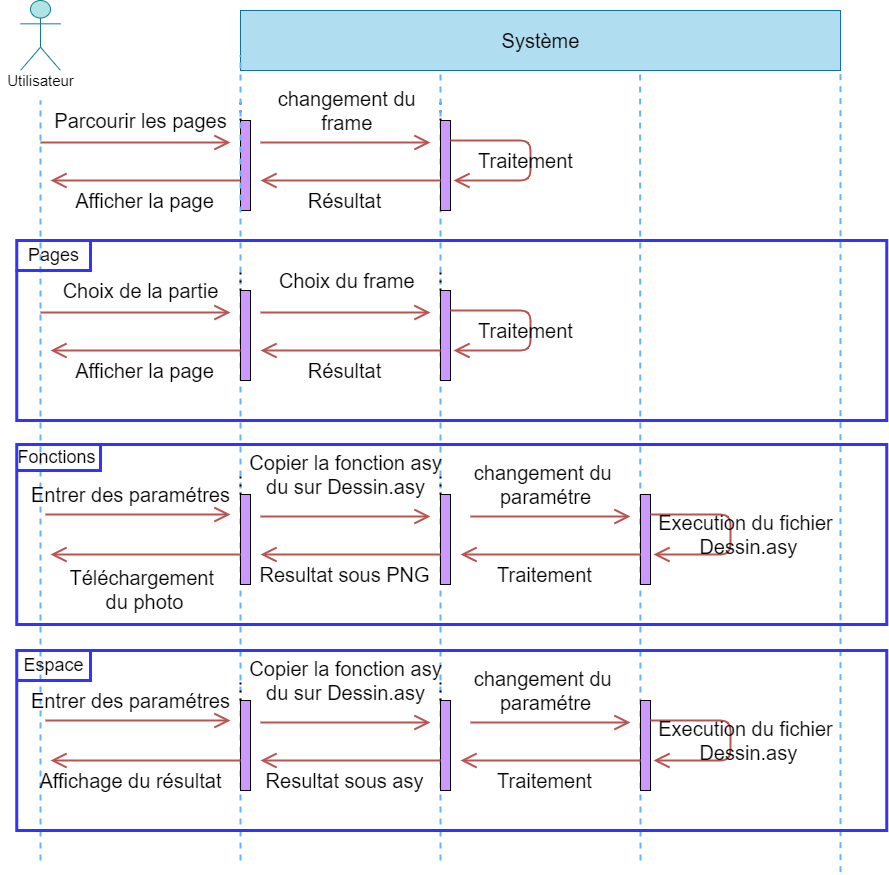
\includegraphics[width=6.6cm]{pic/DS (1).png}
\end{center}
\end{frame}
\section{Étude technique}
\subsection{Environnements de travail}
\begin{frame}{Environnements de travail}
Lors du développement de notre application, nous avons utilisé des différents technologies,outils logiciels et des langages de programmations et qui sont présentés comme suit :
\end{frame}
\begin{frame}{Visual studio code}
\begin{itemize}
\item Visual studio code: Afin d’avoir une bonne aide au développement ainsi qu’une bonne intégration des différents outils de python, Visual Studio Code fut utilisé tout au long du développement de notre application EasyGio.
\end{itemize}
 \begin{center}
     
\includegraphics[width=1.5cm]{pic/Visual Studio Code logo.png}
 \end{center}
\end{frame}
\begin{frame}{Miktex et Microsoft Office }
\begin{itemize}
\item Miktex: C'est une distribution TeX libre pour Windows visant à fournir un environnement TeX/LaTeX complet et prêt à utiliser, pour exécuter les fichier asymptote et rédiger le rapport et la présentation.
\begin{center}
    
\includegraphics[width=2cm]{pic/Miktex.png}
\end{center}\pause
\item Microsoft Office : World 2019 pour la rédaction du cahier des charges.
\begin{center}
    
\includegraphics[width=1.5cm]{pic/Microsoft Office.png}
\end{center}
\end{itemize}
\end{frame}
\begin{frame}{Gantter project et Adobe}
\begin{itemize}
\item Gantter project : Pour la rédaction du diagramme gant.
\begin{center}
    
\includegraphics[width=4cm]{pic/gantter.png}
\end{center}\pause
\item Adobe : Utilisé pour le traitement des images utilisées tout le long du projet que ce soit dans la conception du logo dans le rapport, élaboration du cahier de charge ou le développement de l’application.
\begin{center}
    
\includegraphics[width=1.5cm]{pic/Adobe.jpg}
\end{center}
\end{itemize}
\end{frame}
\subsection{Langages de programmation et technologies utilisés}
\begin{frame}{Asymptote et Git}
Durant notre travail, on a utiliser plusieurs outils et technologies :\pause
\begin{itemize}
\item Asymptote : C'est le Langage de programmation utilisé pour les dessins géométrique pour notre application. 
\begin{center}
    
\includegraphics[width=2cm]{pic/asylogo.png}
\end{center}\pause
\item Git : Pour la gestion de version, étant habitué à Git. Cet outil nous a permis tout au long du PFE de garder trace des différentes évolutions de celui-ci.
\begin{center}
    
\includegraphics[width=2cm]{pic/git.png}
\end{center}
\end{itemize}
\end{frame}
\begin{frame}{Python et son interface graphique}
\begin{itemize}
\item Python : Ses structures de données intégrées de haut niveau, associées à un typage dynamique et à une liaison dynamique, le rendent très attractif pour le développement rapide d'applications, ainsi que pour une utilisation d'interface graphique en utilisant la bibliothèque Tkinter le meilleur choix pour une application graphique simple rapide et facile à utiliser.
\end{itemize}
\end{frame}
\section{Réalisation et résultats}
\begin{frame}{Interface d'accueil}
\begin{center}
    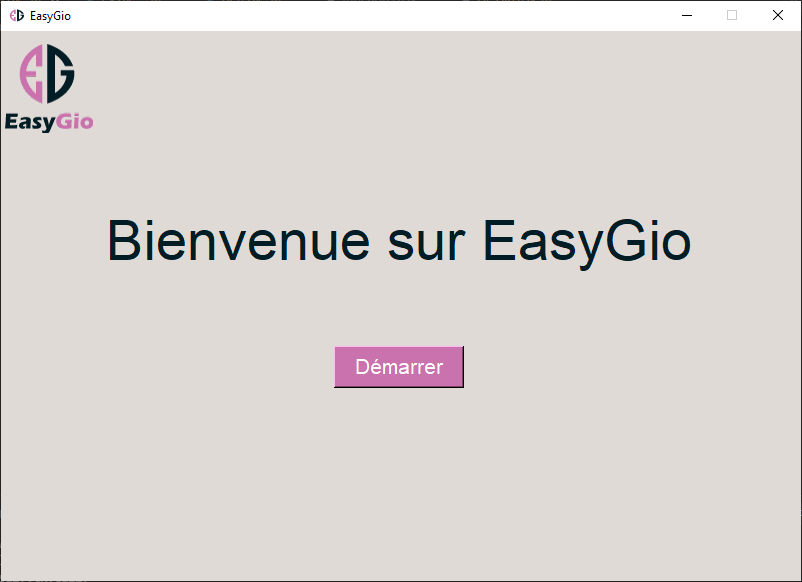
\includegraphics[width=9cm]{pic/Interface1.PNG}
\end{center}
\end{frame}
\begin{frame}{Interface de choix de section}
\begin{center}
    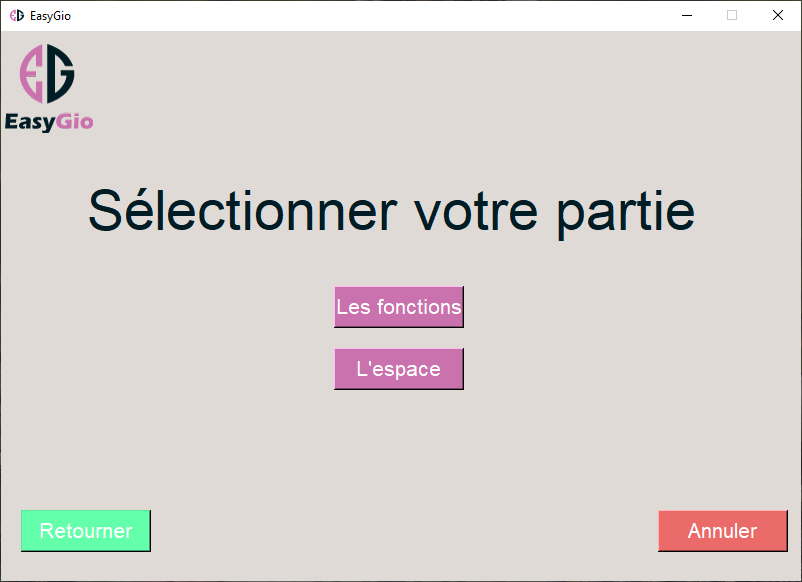
\includegraphics[width=9cm]{pic/Interface2.PNG}
\end{center}
\end{frame}
\begin{frame}{Interfaces de choix des sous parties}
\begin{center}
    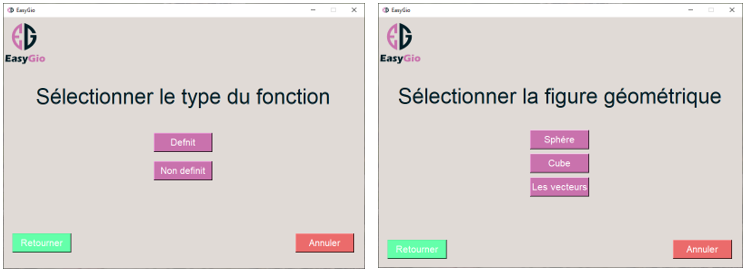
\includegraphics[width=11cm]{pic/TypesCaptures.PNG}
\end{center}
\end{frame}
\begin{frame}{Interfaces des insertion des paramètres}
\begin{center}
    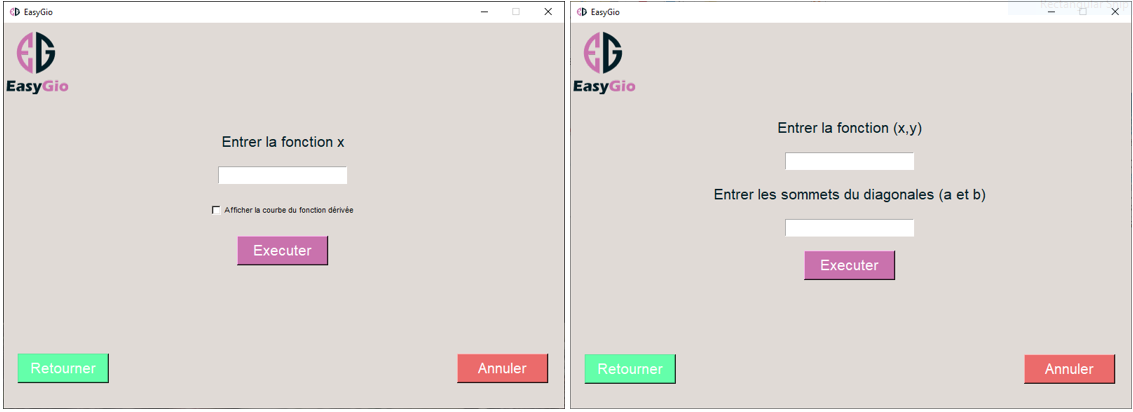
\includegraphics[width=11cm]{pic/InputesInter.PNG}
\end{center}
\end{frame}
\begin{frame}{Exécution d'une fonction (Courbe)}
\begin{center}
    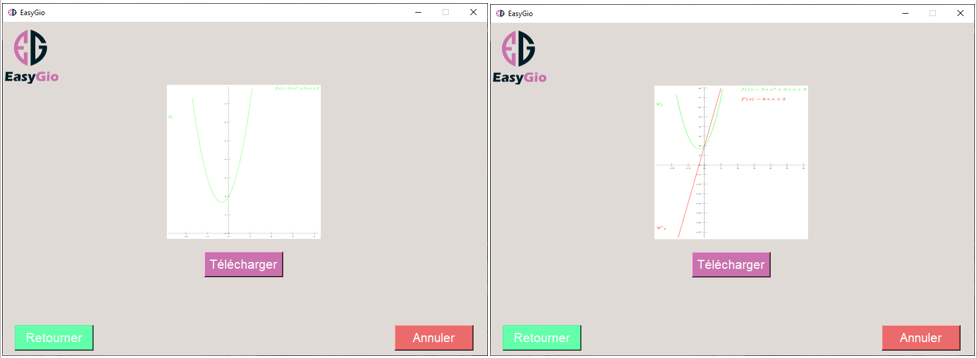
\includegraphics[width=11cm]{pic/Fonction.PNG}
\end{center}
\end{frame}
\begin{frame}{Interfaces de Sphère et de Cube}
\begin{center}
    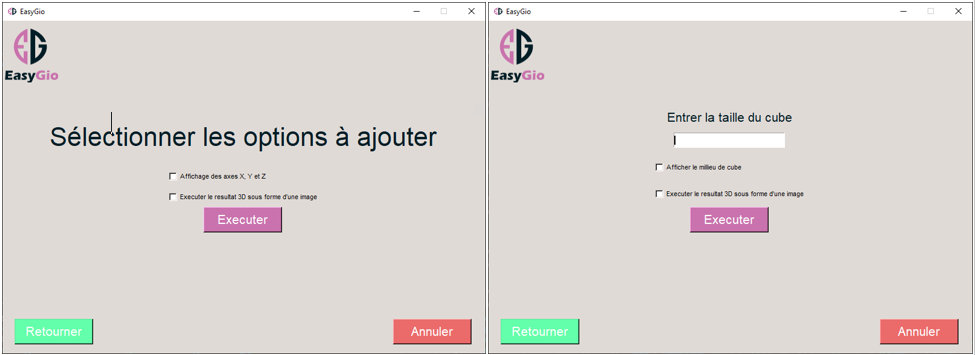
\includegraphics[width=11cm]{pic/SpCube.PNG}
\end{center}
\end{frame}
\begin{frame}{Erreur de nombre non entier}
\begin{center}
    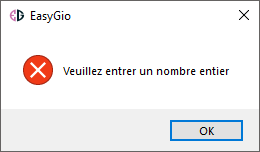
\includegraphics[width=9cm]{pic/NbError.PNG}
\end{center}
\end{frame}
\begin{frame}{Transférer le résultat 3D à une image}
\begin{center}
    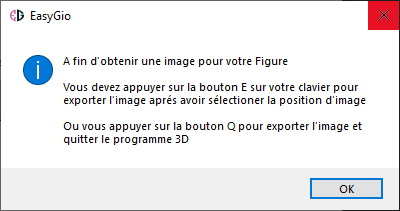
\includegraphics[width=9cm]{pic/3DToImage.PNG}
\end{center}
\end{frame}
\begin{frame}{Exécution d'une figure 3D (cube)}
\begin{center}
    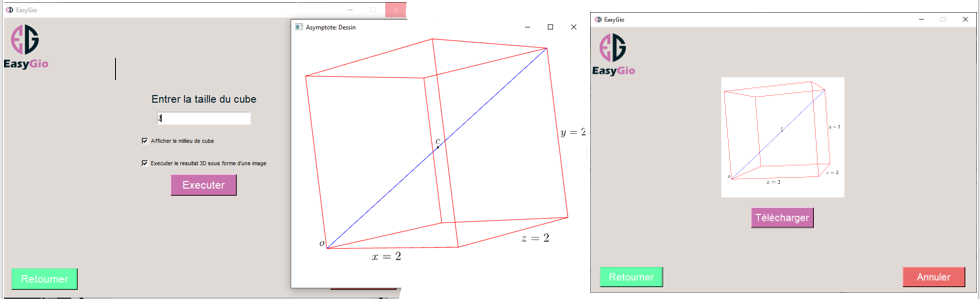
\includegraphics[width=11cm]{pic/CubeT.PNG}
\end{center}
\end{frame}
\begin{frame}{Interface de choix des figures pour les vecteurs}
\begin{center}
    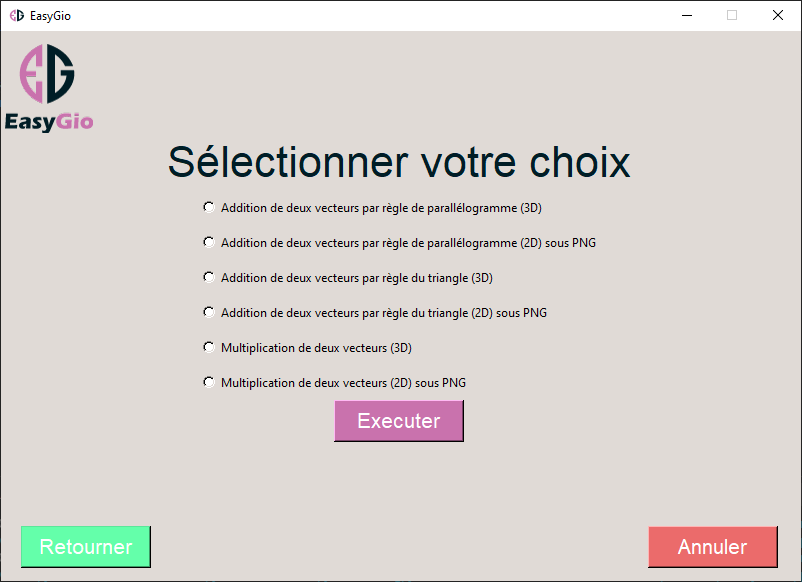
\includegraphics[width=9cm]{pic/Vecteur.PNG}
\end{center}
\end{frame}
\begin{frame}{Choix d'emplacement de téléchargement du fichier}
\begin{center}
    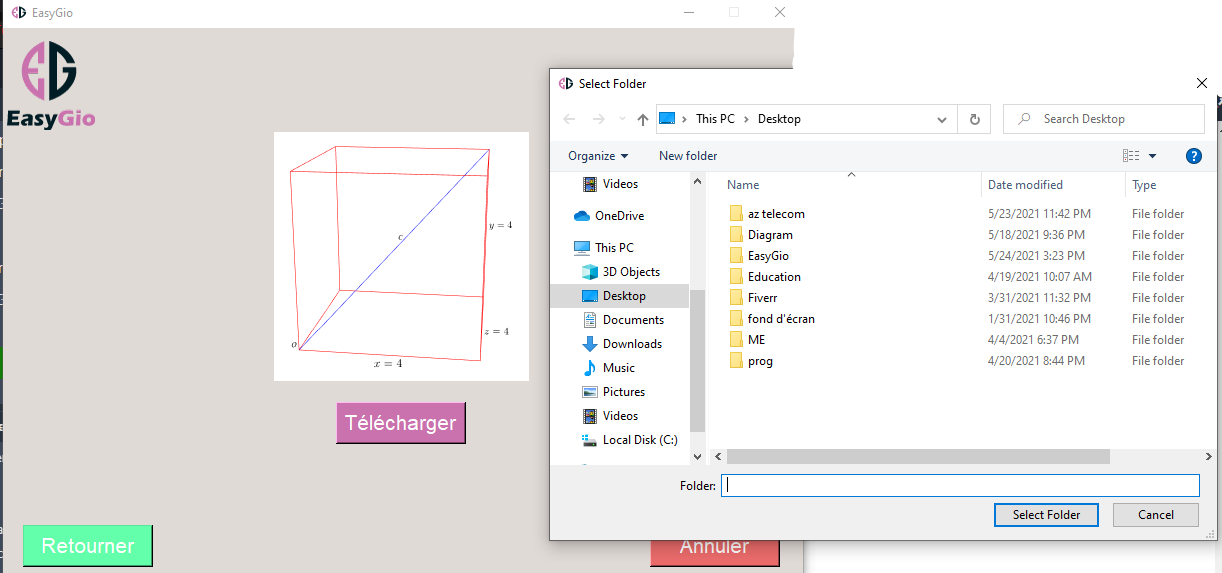
\includegraphics[width=11cm]{pic/CubeP.PNG}
\end{center}
\end{frame}
\begin{frame}{EasyGio Info et Erreur fenêtres}
\begin{center}
    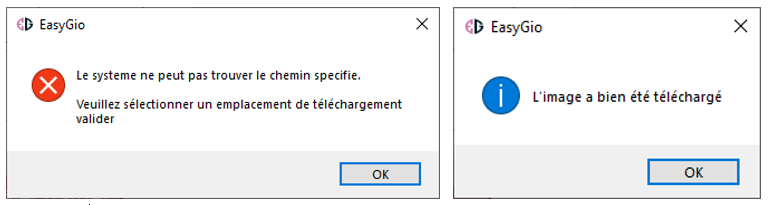
\includegraphics[width=11cm]{pic/nots.PNG}
\end{center}
\end{frame}
\section{Conclusion}
\begin{frame}{Conclusion}
\note{%
Malgré les difficultés rencontrées durant ce projet et en particulier le fait de traiter un sujet d’actualité avec peu de documentation, nous sommes parvenues à nous familiariser avec ces nouvelles technologies liées au Asymptote, et crée une application qui va très faciliter l'illustration des notions de géométrie pour les enseignants et ces élevés et de construire des multiple figures rapidement et en simple clics et surtout dans l'espace à travers notre système des figures 3D.
}
Malgré les difficultés rencontrées durant ce projet et en particulier le fait de traiter un sujet d’actualité avec peu de documentation, nous sommes parvenues à nous familiariser avec ces nouvelles technologies liées au Asymptote, et crée une application qui va très faciliter l'illustration des notions de géométrie pour les enseignants et ces élevés et de construire des multiple figures rapidement et en simple clics et surtout dans l'espace à travers notre système des figures 3D.
\end{frame}
\begin{frame}
    \begin{center}
        {\Huge\calligra Merci Pour Votre Attention!}
    \end{center}
\end{frame}

\end{document}